This section section describes the results of different measurements, calculations and tests that were run on the Barricelli computer.
It also documents the different demonstration programs that showcase and illustrate Barricelli's purpose through practical use, as well as research done in the design of Barricelli.

\section{Research}

\subsection{Steady State Genetic Algorithm}
A big question in the design of the architecture, was how to implement the genetic algorithm.
As \vref{fr7} states, the instruction set should include instructions to speed up genetic operations.
To fulfill this requirment, the algorithm would have to be directly integrated with the computer.

In the research, some papers were found that discussed Steady State Genetic Algorithms.\cite{vlsi-ga}
As these were described as being advantageous on a MIMD architecture, there was interest in further research.
However, few citations were found on how steady state algorithms performancewise related to traditional genetic algorithms.
This section documents an original research on Steady State, where both a generational and a steady state solver was implemented in Python, and used to solve a problem.

\subsubsection{Problem}
\lstinputlisting[language=Python, caption={Genetic problem}, label={lst:problem}]{continuous-ga-test/problems.py} 

The problem, implemented in listing \ref{lst:problem}, is to maximize a bit string, that is to make let have every bit be 1.
Implemented are functions for selection, crossover, mutation, creation and calculating fitness.
I. e. what is needed for a genetic search.

\subsubsection{Solvers}
\lstinputlisting[language=Python, caption={Generational solver}, label={lst:gensolver}, firstline=3, lastline=59]{continuous-ga-test/solvers.py} 

\lstinputlisting[language=Python, caption={Steady state solver}, label={lst:steadsolver}, firstline=62, lastline=108]{continuous-ga-test/solvers.py} 

In listing \ref{lst:gensolver}, there is implemented a generational version of a genetic algorithm, while in listing \ref{lst:steadsolver} there is a steady state version.
The main difference of these two solvers is how the new individuals are added to the population.
In the generational, the new individuals are inserted for the worst individuals in the old population, maintaining the population size by keeping the best of the old population if there is not enough new individuals.
The steady state version just replaces a random selected individual of the current population with the new one.

\subsubsection{Result}
\begin{table}[H]
\begin{center}
\begin{tabular}{ | c | c | }
    \hline
    Generational    & Steady State \\
    \hline
    210             & 10899 \\
    243             & 27714 \\
    238             & 2336  \\
    134             & 4210  \\
    223             & 2048  \\
    143             & 4365  \\
    285             & 1526  \\
    244             & 8733  \\
    141             & 21515 \\
    180             & 3119  \\
    \hline
\end{tabular}
\end{center}
\caption{Results of ten runs of the genetic programs}
\label{tbl:genresults}
\end{table}
After 10 runs, the generational implementation had average number of generations equal 204.1, while the steady state has a comparative result of 86.5.
The result of the steady state seems much higher than the generational, as it doesn't count generation in the same way.
To get comparable results, the work of the steady state algorithm should be divided by the population size, in this case 100.

As can be seen from table \ref{tbl:genresults}, the number of generations varies a lot more in the steady state, but as the average was significantly lower than generational, the conclusion was that steady state was better, and chosen for the project.


\section{Measurements}

This section presents the measurements found during the project.
These results are discussed in Chapter \vref{chapter:discussion}.

\subsection{Performance}

\begin{figure}[H]
    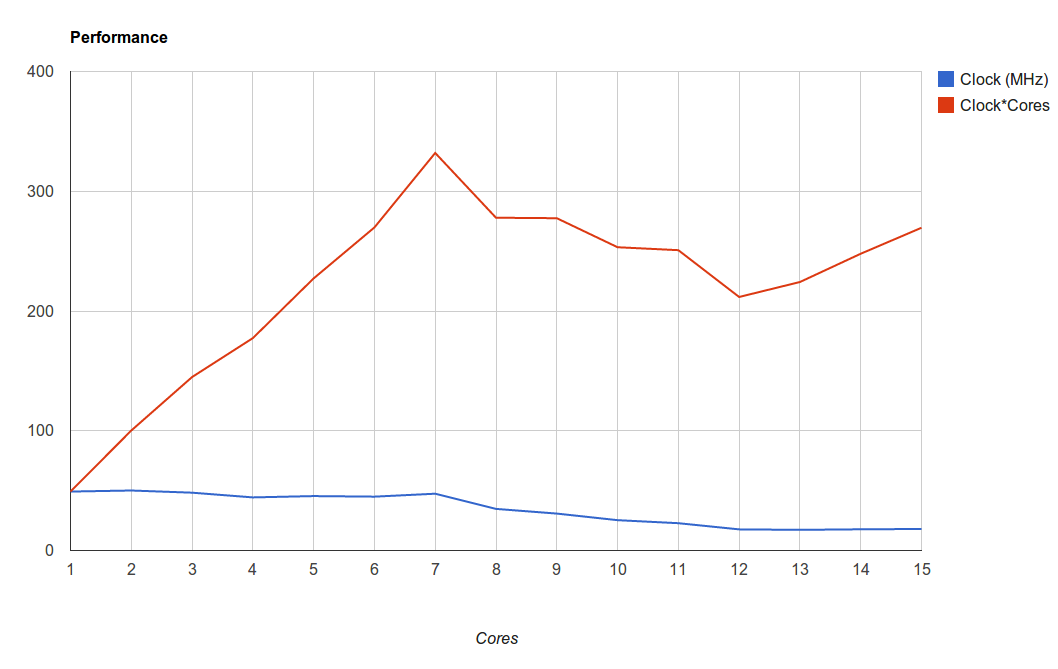
\includegraphics[width=\textwidth]{fpga/fig/performance.png}
    \caption{Total performance of Barricelli's fitness cores, as a function of number of cores}
    \label{figure:total-performance}
\end{figure}

The total performance of Barricelli's fitness cores, measured as maximum theoretical clock speed times number of clock cores, is illustrated in Figure \vref{figure:total-performance}.
This 

\todo{measure performance with different core amounts}

\todo{measure performance with and without genetics pipeline}

\todo{measure performance of same problems on consumer grade laptop}

\todo{measure performance of general program}



\section{Demonstration Programs}

This section documents the demonstration programs written for the Barricelli computer to demonstrate its functionality.
The programs are typically written in \gls{galapagos} assembly for programs running on the custom processor, and C for programs running on the \Gls{SCU}.
The source code for these demonstration programs can be found in appendix \vref{appendix:demonstration-programs-source-code}.

\subsection{Genetic Algorithm: Color Search}

The color search program is a very simple program demonstrating a basic usage of the genetics accelerator.
The program tries to find a specific color in the search-space of all 24-bit colors.

\subsubsection{Individual representation}

An individual represents a specific 24-bit color in RGB format.
The individual is coded to a 64-bit data word like in figure \vref{figure:color-search-bytefield}.

\begin{figure}[H]
    \begin{center}
        \begin{bytefield}[bitwidth=0.5em,endianness=big]{64}
            \bitheader[bitformatting={\tiny\rotatebox[origin=B]{90}}]{0, 7, 8, 15, 16, 23, 24, 63} \\
        \bitbox{40}{\color{lightgray}\rule{\width}{\height}}
            \bitbox{8}{blue}
            \bitbox{8}{green}
            \bitbox{8}{red}
        \end{bytefield}
        \caption{The binary coding of an individual for the color search problem}
        \label{figure:color-search-bytefield}
    \end{center}
\end{figure}

\subsubsection{Fitness Function}

The fitness for an individual is calculated using equation \vref{equation:color-search-fitness-function}.
The fitness a any given individual falls in the range $ [0, 768] $.

\begin{eqnarray}
\nonumber
fitness & = & 768 \\
\nonumber
        & - & |red_{individual} - red_{target}| \\
\nonumber
        & - & |green_{individual} - green_{target}| \\
        & - & |blue_{individual} - blue_{target}|
\label{equation:color-search-fitness-function}
\end{eqnarray}

\subsubsection{Results}

Figure \vref{figure:color-search} shows the evolution of the approximation suggested as an answer by the genetic algorithm.
In this problem instance the target color was magic pink, i.e. the color with color code $ rgb(255, 0, 255) $.
The program run illustrated in figure \vref{figure:color-search} ran on 7 seven cores, and the measurements are from regularly polling a single core for its current best solution.
Figure \vref{figure:color-search} clearly illustrates a typical trait of genetic algorithm approximations: they are quite good at finding decent approximations, but iterating to improve accuracy of the result is a game of diminishing returns.
The algorithm quickly finds a decent approximation of the target color, but finding the exact value down to the last bit still takes time.

\begin{figure}[H]
    \begin{center}
        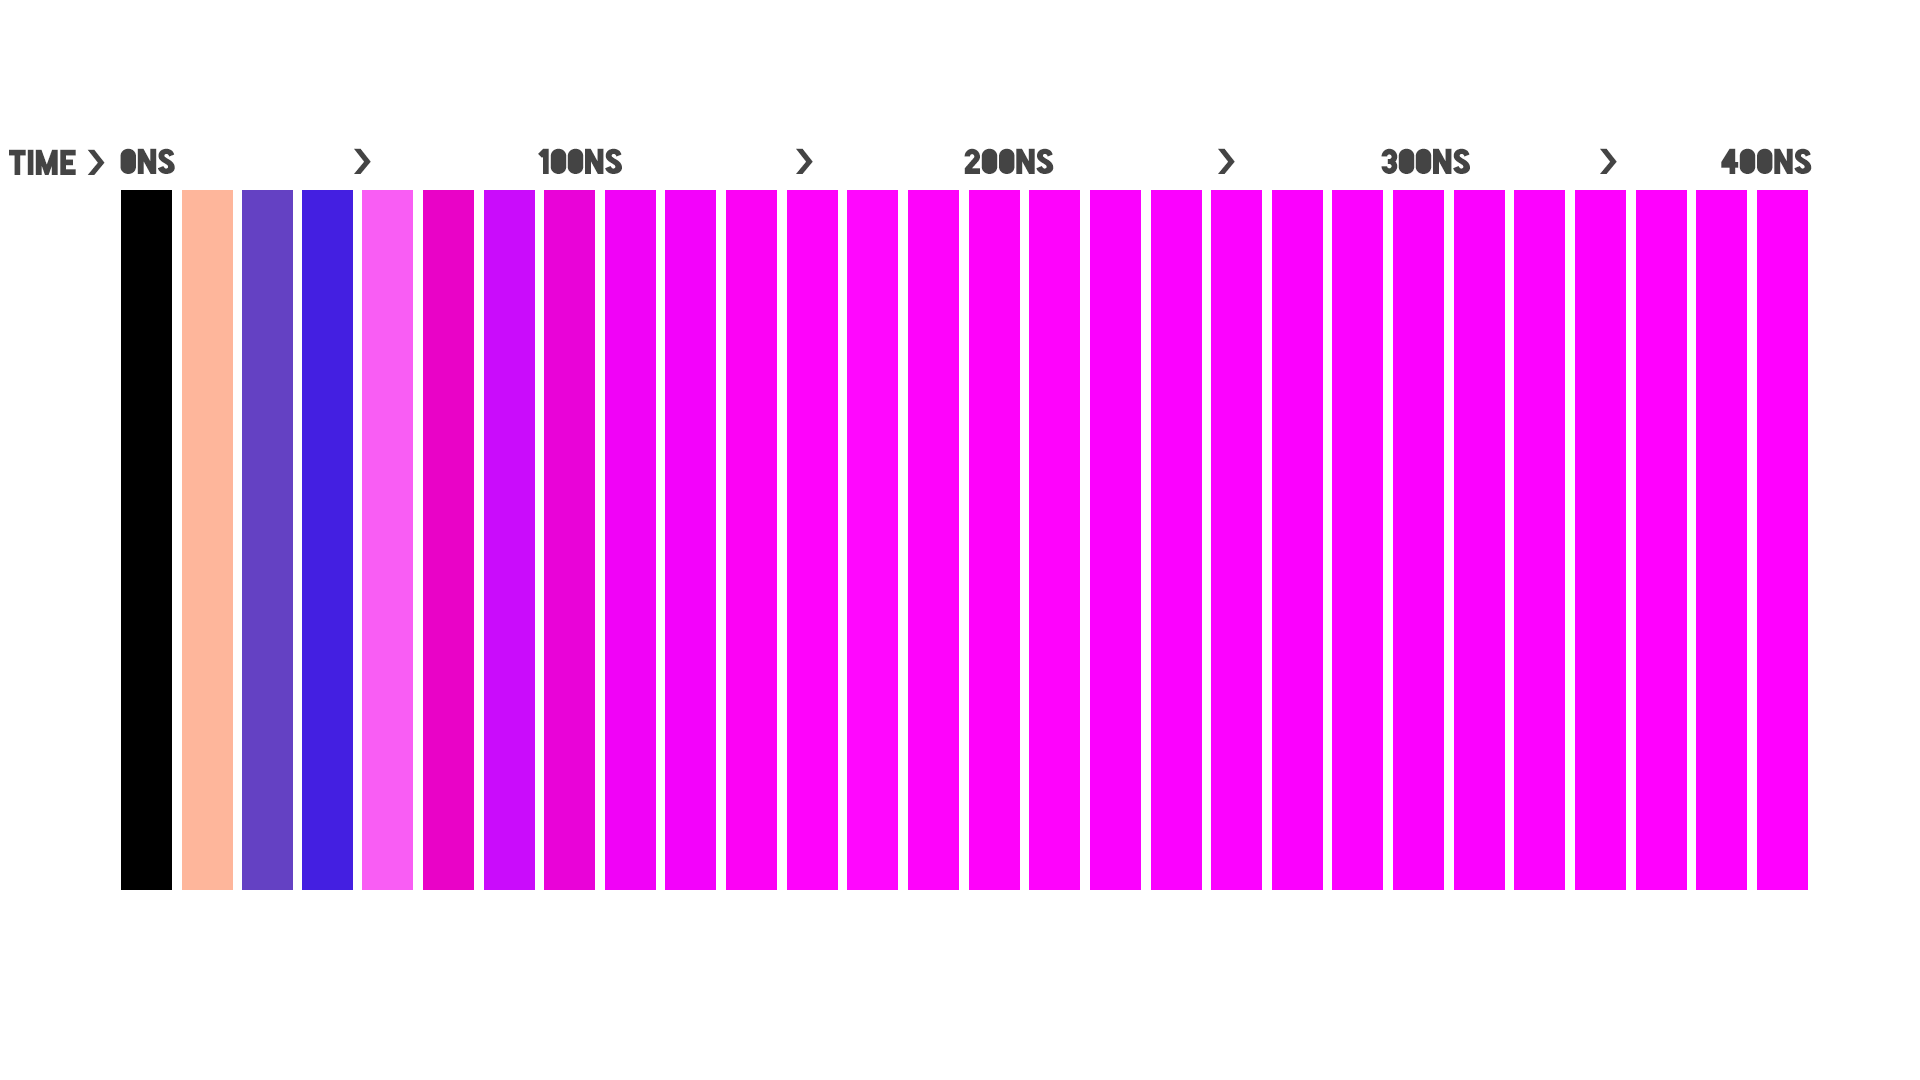
\includegraphics[width=\textwidth]{fig/color-search}
    \caption{Color search progression (7 cores, 1 core sampled)}
    \label{figure:color-search}
    \end{center}
\end{figure}

\subsection{Genetic Algorithm: Binary Knapsack Problem}

The knapsack problem is an optimization problem that is considered NP-hard.
The problem to solve is given a set of items with a weight and a value and a knapsack that can hold a specific weight, what combination of items that can fit in the sack has the highest value.
If there can be at most one of each item in the knapsack, we have what is known as the binary knapsack problem.

\subsubsection{Individual representation}

An individual represents a combination of items.
The individual is coded to a 64-bit data word like in Figure \vref{figure:binary-knapsack-bytefield}.

\begin{figure}[H]
    \begin{center}
        \begin{bytefield}[bitwidth=0.5em,endianness=big]{64}
            \bitheader{0, 63} \\
            \bitbox{63}{bit $ i $ set if item $ i $ is in the include set, else unset}
        \end{bytefield}
        \caption{The binary coding of an individual for the binary knapsack problem}
        \label{figure:binary-knapsack-bytefield}
    \end{center}
\end{figure}

\subsubsection{Fitness Function}
The fitness for an individual is calculated using Algorithm \ref{algorithm:binary-knapsack-fitness-function}.
The fitness falls between 0 for invalid sacks (that contain too much weight) to a theoretical maximum of the sum of the value of all the items.

\begin{algorithm}[H]
\SetAlgoLined
\DontPrintSemicolon
\KwData{A bit array with one bit representing whether each item is included or not}
\KwResult{How fit the individual is}
\Begin{
    $ weight \longleftarrow 0$\;
    $ value \longleftarrow 0$\;
    \For {item in ItemSet} {
        \If {item in genome} {
            $ weight \longleftarrow weight + item.weight$\;
            $ value \longleftarrow value + item.value$\;

            \If {$weight > maxWeight$} {
                $ value \longleftarrow 0$\;
                $ break $\;
            }
        }
    }
    \;
    \Return{$ value $}
}
\caption{The fitness function for the binary knapsack problem}
\label{algorithm:binary-knapsack-fitness-function}
\end{algorithm}

\subsubsection{Results}

This problem has not been run on the actual hardware, only simulated up to a few milliseconds.
The simulation seemed fine, and we got increasing fitness values, but the problem space is huge, so we probably need to run the algorithm for quite some time before coverging to a ideal/near-ideal solution.

\subsection{Blinkenlights}
Blinkenlights is a program that demonstrates the use of the input and output of the \Gls{barricelli} driven by the \Gls{SCU}.
When a button is pressed, the corrensponding LEDs to the button lit up.
This program is also described as a test for I/O, in \vref{iotest}, named Buttons \& LEDs.

